\documentclass[aspectratio=169]{beamer}
\mode<presentation>
%\usetheme{Warsaw}
%\usetheme{Goettingen}
\usetheme{Hannover}
%\useoutertheme{default}

%\useoutertheme{infolines}
\useoutertheme{sidebar}
\usecolortheme{dolphin}


\setbeamersize{sidebar width left=0pt} % to remove the sidebar
\beamertemplatenavigationsymbolsempty % To remove the navigation symbols on the bottom right.
\setbeamersize{text margin left=10mm,text margin right=10mm} % Specify margins

\usepackage{amsmath}
\usepackage{amssymb}
\usepackage{listings}
\usepackage{enumerate}
\usepackage{hyperref}
\hypersetup{
    colorlinks=true,
    linkcolor=blue,
    filecolor=magenta,      
    urlcolor=cyan,
}

%%%%For drawing graphs
% a nice font
\usepackage{kpfonts}

% basic text stuff
\usepackage[utf8]{inputenc}
\usepackage[T1]{fontenc}

\usepackage{tikz} % main tikz package
\usepackage{tikz-network} % for network / graph utilities

% for a nicer colorscheme
%\input{colors.tex} % By nemo.fournier https://nemo.kiwi/latex.html#h3_colors
%%%%%%%%%%%%%%%%%%%%%%%%%%%%%%%

\begin{document}
 
\urlstyle{same}

%some bold math symbosl
\newcommand{\Cov}{\mathrm{Cov}}
\newcommand{\Var}{\mathrm{Var}}
\newcommand{\brho}{\boldsymbol{\rho}}
\newcommand{\bSigma}{\boldsymbol{\Sigma}}
\newcommand{\btheta}{\boldsymbol{\theta}}
\newcommand{\bbeta}{\boldsymbol{\beta}}
\newcommand{\bmu}{\boldsymbol{\mu}}
\newcommand{\bW}{\mathbf{W}}
\newcommand{\one}{\mathbf{1}}
\newcommand{\bH}{\mathbf{H}}
\newcommand{\by}{\mathbf{y}}
\newcommand{\bolde}{\mathbf{e}}
\newcommand{\bx}{\mathbf{x}}

\newcommand{\cpp}[1]{\texttt{#1}}

%--------------------------------------------------
\providecommand{\abs}[1]{\lvert#1\rvert}
\providecommand{\norm}[1]{\lVert#1\rVert}
\providecommand{\Blue}[1]{\textcolor{blue}{#1}}
\providecommand{\Red}[1]{\textcolor{red}{#1}}  
\providecommand{\Purple}[1]{\textcolor{purple}{#1}} %for notations
\newcommand{\celsius}{\ensuremath{^\circ}C}
\newcommand\thfore{\mathord{\therefore}\,}
%------------------------------------------------------------------

\title{Lecture 5. Euler Paths and Circuits}
%\author{
\includegraphics[width=.8\textwidth,height=.7\textheight]{lecture1-fig0.jpg}}

\date{ }
%------------------------------------------------------------------

\frame[plain]{\titlepage}

\begin{frame}[plain]{} 


\begin{center}
  {\bf Does a path or circuit exist that uses every edge exactly once?
  }
\end{center}

\vspace{.3in}

\begin{columns}[t] % contents are top vertically aligned
\begin{column}[c]{5cm}

%%%Sample code for drawing is after \end{document}
  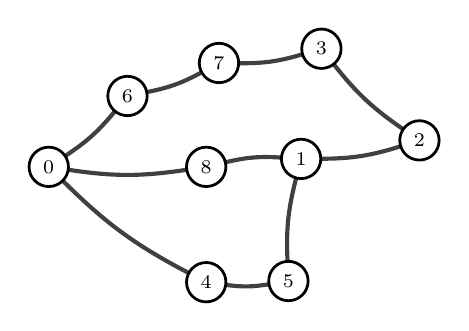
\begin{tikzpicture}[>=stealth']
 %   \coordinate (13) at (3.572,1.845);
    
    \Vertex[color=white,x=0.646,y=4.250,size=0.5,label=0]{0}
    \Vertex[color=white,x=3.851,y=4.351,size=0.5,label=1]{1}
    \Vertex[color=white,x=5.354,y=4.586,size=0.5,label=2]{2}
    \Vertex[color=white,x=4.109,y=5.750,size=0.5,label=3]{3}
    \Vertex[color=white,x=2.646,y=2.785,size=0.5,label=4]{4}
    \Vertex[color=white,x=3.690,y=2.800,size=0.5,label=5]{5}    
    \Vertex[color=white,x=1.646,y=5.150,size=0.5,label=6]{6} 
    \Vertex[color=white,x=2.808,y=5.569,size=0.5,label=7]{7}
    \Vertex[color=white,x=2.646,y=4.250,size=0.5,label=8]{8}
        
    \Edge[,bend=-8.531](0)(6)
    \Edge[,bend=-8.531](0)(8)
    \Edge[,bend=-8.531](0)(4)
    \Edge[,bend=-8.531](6)(7)
    \Edge[,bend=-8.531](7)(3)
    \Edge[,bend=-8.531](3)(2)
    \Edge[,bend=-8.531](1)(2)
    \Edge[,bend=-8.531](1)(8)
    \Edge[,bend=-8.531](1)(5)
    \Edge[,bend=-8.531](4)(5)
    
    
   \end{tikzpicture}    
   
  \end{column} \pause
  \begin{column}[c]{5cm}
     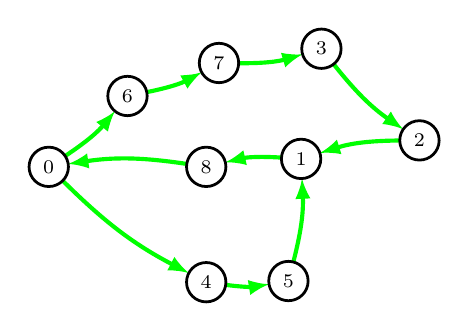
\begin{tikzpicture}[>=stealth']
 %   \coordinate (13) at (3.572,1.845);
 
    \Vertex[color=white,x=0.646,y=4.250,size=0.5,label=0]{0}
    \Vertex[color=white,x=3.851,y=4.351,size=0.5,label=1]{1}
    \Vertex[color=white,x=5.354,y=4.586,size=0.5,label=2]{2}
    \Vertex[color=white,x=4.109,y=5.750,size=0.5,label=3]{3}
    \Vertex[color=white,x=2.646,y=2.785,size=0.5,label=4]{4}
    \Vertex[color=white,x=3.690,y=2.800,size=0.5,label=5]{5}    
    \Vertex[color=white,x=1.646,y=5.150,size=0.5,label=6]{6} 
    \Vertex[color=white,x=2.808,y=5.569,size=0.5,label=7]{7}
    \Vertex[color=white,x=2.646,y=4.250,size=0.5,label=8]{8}
        
    \Edge[color=green,Direct,bend=-8.531](0)(6)
    \Edge[color=green,Direct,bend=-8.531](8)(0)
    \Edge[color=green,Direct,bend=-8.531](0)(4)
    \Edge[color=green,Direct,bend=-8.531](6)(7)
    \Edge[color=green,Direct,bend=-8.531](7)(3)
    \Edge[color=green,Direct,bend=-8.531](3)(2)
    \Edge[color=green,Direct,bend=-8.531](2)(1)
    \Edge[color=green,Direct,bend=-8.531](1)(8)
    \Edge[color=green,Direct,bend=-8.531](5)(1)
    \Edge[color=green,Direct,bend=-8.531](4)(5) 
    
   \end{tikzpicture}    
  \end{column}
  \end{columns}
\vspace{.3in}


\begin{itemize}
           \item An \Blue{Euler path} in a graph $G$ is a \Red{simple path} {\bf containing 
              every edge of $G$}. That is, an Euler path is a path that
              visits every edge exactly once (allowing for revisiting vertices).
           \item An \Blue{Euler circuit} in a graph $G$ is 
           an Euler path that starts and ends on the same vertex.
          \end{itemize}
    
\end{frame}


\begin{frame}[plain]{}

[\href{https://twitter.com/brilliantorg/status/1175031964727959558}{The Bridges of Königsberg }]. 
    K\"{o}nigsberg is the name for the historic Prussian city that is now Kaliningrad, Russia.
    The town had a river with two islands. The islands were connected to the river banks by seven bridges 
    (see below).
     There was an 
entertaining or interesting exercise for the citizens 
of Konigsberg. \Blue{ Start from any land regions and 
come back to the starting point after crossing each 
of the seven bridges exactly once without repeating 
same path. Is it possible?}
       The Swiss mathematician Leonhard Euler solved this problem~\footnote{
  \href{https://www.maa.org/press/periodicals/convergence/leonard-eulers-solution-to-the-konigsberg-bridge-problem}{Leonard Euler's Solution to the Konigsberg Bridge Problem}}
       in 1736. Can you solve it?
      \begin{center}
     %   \includegraphics[height=4cm]{../Lecture_S15/lecture7-fig0.png}
     \href{https://twitter.com/brilliantorg/status/1175031964727959558}
        {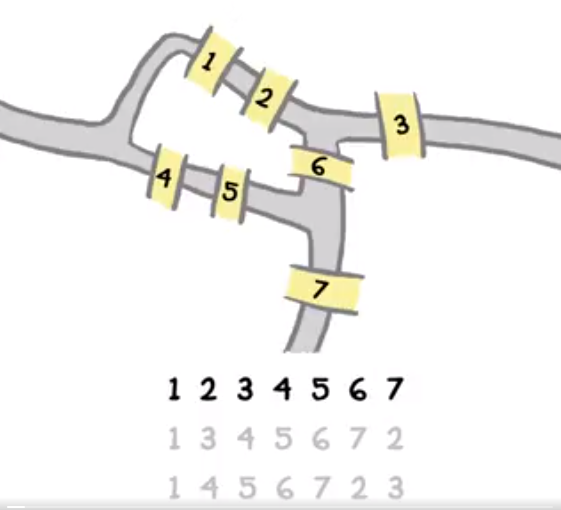
\includegraphics[height=4cm]{./img/lecture5-fig1.png}}
      \end{center}
     

\end{frame}

\begin{frame}[plain]{}

    
     The problem of traveling across every bridge without crossing any bridge more than once
can be rephrased in terms of this graph model. 
   

   \begin{columns}[t] % contents are top vertically aligned
        \begin{column}[c]{5cm}
          \begin{center}
         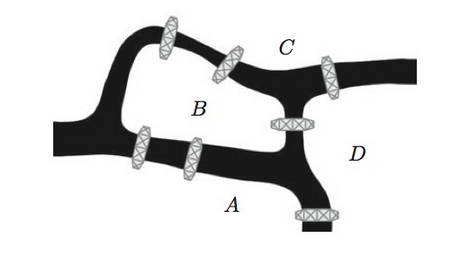
\includegraphics[height=3.5cm]{./img/lecture5-fig2.png}
       \end{center}
        \end{column}
       \begin{column}[c]{5cm} % each column can also be its own environment           
             \begin{center}
        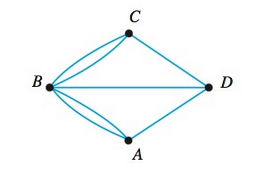
\includegraphics[height=3.5cm]{./img/lecture5-fig3.png}
      \end{center}           
        \end{column}
  \end{columns}  
  \medskip
  
We can rephrase the question like:
\begin{center}
 \Blue{Is there a simple  
circuit in this
graph that contains every edge?}
 \end{center}
 Equivalently, \Blue{does this graph contain an Euler circuit?}
 
\end{frame}

\begin{frame}[plain]{}
 
 
   \begin{columns}[t] % contents are top vertically aligned
        \begin{column}[c]{2.5cm}           
          \begin{center}
         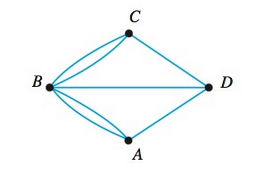
\includegraphics[height=3cm]{./img/lecture5-fig3.png}
       \end{center}
        \end{column}
       \begin{column}[c]{8.5cm} % each column can also be its own environment           
          \begin{enumerate}[<+->]
           \item In any graph $G = (V,E)$, the sum of the \emph{degree of the vertices} 
             equals twice the \emph{number of of edges}, because each edge 
             contributes 2 to the sum of the degrees:
             \[ \Blue{\sum_{v\in V}deg(v) = 2\,|E| }\]
             where $|E| = $ the number of edges in $G$.
           \item If all the vertices of a connected graph have even degree,
              then the graph has an \Blue{Euler circuit}.
           \item If a connected graph has exactly two vertices, $v$ and $w$, of odd degree,
             then there is an \Blue{Euler path} from $v$ to $w$.
           \item If a graph has more than two \emph{vertices} of odd degree, it does not
              have an Euler path.
          \end{enumerate}
           
        \end{column}
  \end{columns}  
     
\end{frame}

\begin{frame}[plain]{Answer: The Seven Bridges of K\"{o}nigsberg}

   \begin{columns}[t] % contents are top vertically aligned
        \begin{column}[c]{5cm}
          \begin{center}
         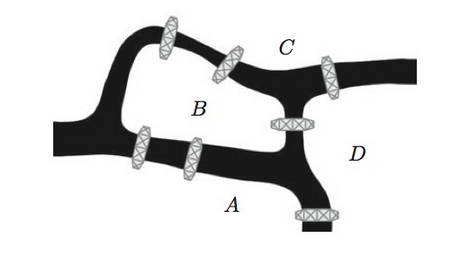
\includegraphics[height=2.7cm]{./img/lecture5-fig2.png}
       \end{center}
        \end{column}
       \begin{column}[c]{5cm} % each column can also be its own environment           
             \begin{center}
        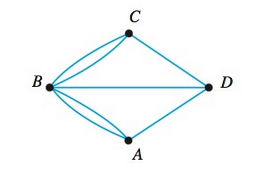
\includegraphics[height=3cm]{./img/lecture5-fig3.png}
      \end{center}           
        \end{column}
  \end{columns}  
  
  The vertices $A, B, C,$ and $D$ of the graph have degrees 3, 5, 3, and 3, respectively. Therefore,
  this graph does not have an Euler path. In the language of bridges, there is no way a connected walk
  can cross each bridge exactly once.
     
\end{frame}

\begin{frame}[plain]{NECESSARY AND SUFFICIENT CONDITIONS FOR EULER CIRCUITS AND PATHS}
  \begin{itemize}
   \item {\bf Theorem 5.1.} A connected graph with at least two vertices has an Euler circuit 
   \Blue{if and only if} each of its vertices has even degree.
      \item {\bf Theorem 5.2.} A connected graph has an Euler path but not an Euler circuit 
      \Blue{if and only if} it has exactly two vertices of odd degree.
  \end{itemize}
\medskip
  
{\bf Example 5.3.}  Does the following graph have an Euler path? Why or why not?
     \begin{center}
        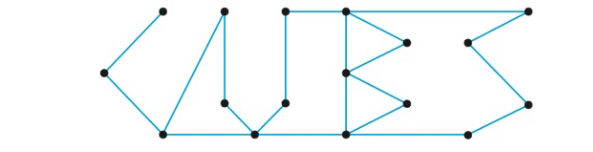
\includegraphics[height=2cm]{./img/lecture5-fig4.png}
      \end{center} 
   
   How many different Euler paths are there in the graph?    
      
\end{frame}

\begin{frame}[plain]{}

{\bf Practice 5.4.} The floor plan shown below is for a house open for public viewing. 
 Is it possible to find a path that starts in room $A$, ends in room $B$, and passes through 
 every \emph{interior} doorway 
 of the house exactly once?
 Illustrate the graph that represents the question and
 determine whether such a path exists on the graph. 

  \begin{center}
        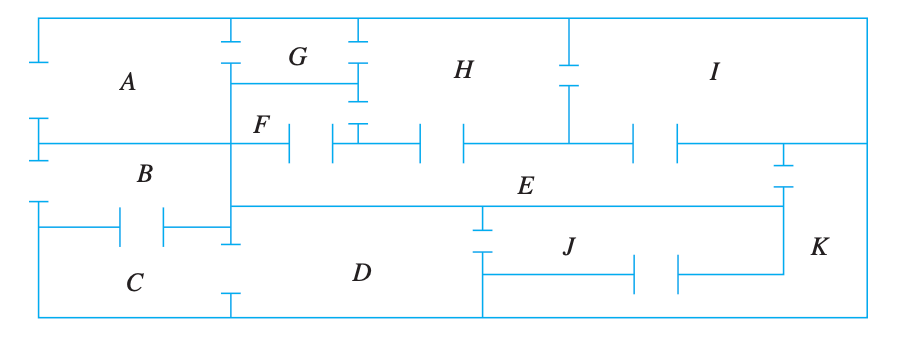
\includegraphics[height=3.3cm]{./img/lecture5-fig5.png}
      \end{center} 

 How many different Euler paths are there in the graph? 
 
 \end{frame}
 
 \begin{frame}[plain]{Fleury’s Algorithm}
 
  Now we know how to determine if a graph has an Euler circuit, but if it does, how do we find one?
  \medskip
  
  \underline{\bf FLEURY'S ALGORITHM}
  \begin{enumerate}
    \item Start at any vertex if finding an Euler circuit. If finding an Euler path, start at one of the two vertices with odd degree.
    \item Choose any edge leaving your current vertex, provided deleting that edge will not separate the graph 
      into two disconnected sets of edges.
   \item Add that edge to your circuit, and delete it from the graph.
   \item Continue until you’re done.
 \end{enumerate}
 
 %Fleury’s Algorithm for printing Eulerian Path or Circuit in Python (including 
 %  algorithm complexity
 %  https://www.geeksforgeeks.org/fleurys-algorithm-for-printing-eulerian-path/
 
 \end{frame}
 
 \begin{frame}[plain]{}
 
 %. https://courses.lumenlearning.com/wmopen-mathforliberalarts/chapter/introduction-euler-paths/
 
  {\bf Example 5.5.} Find an Euler Circuit on this graph using Fleury's algorithm, starting at vertex $A$.
     \begin{center}
        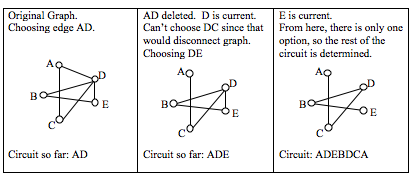
\includegraphics[height=4.5cm]{./img/lecture5-fig6.png}
      \end{center} 

\end{frame}

\begin{frame}[plain]{}
 
 %. https://courses.lumenlearning.com/wmopen-mathforliberalarts/chapter/introduction-euler-paths/
 %  https://math.libretexts.org/Bookshelves/Applied_Mathematics/Math_in_Society_(Lippman)/06%3A_Graph_Theory/6.05%3A_Eulerization_and_the_Chinese_Postman_Problem
 
  {\bf Activity 5.6.} Consider the graph
   \begin{center}
        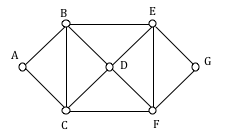
\includegraphics[height=3cm]{./img/lecture5-fig7.png}  \ \ \ \ \ \ \ \ \ \  \ \ \ \ \ \ \ \ \ \ \ \ \ \ \ \ \ \ \ \ \ \ \ \ \ \ \ \ \ 
      \end{center} 
  \begin{itemize}
    \item[(a)]
  Does the graph have an Euler Circuit? 
   If so, find one using Fleury's algorithm.
   (Visualize each step of solving.)
   \item[(b)] How many different Euler circuits are there in this graph?
 \end{itemize}
 %Ref:  
 %https://math.stackexchange.com/questions/2057570/how-many-different-eulerian-circuits-are-there-in-this-graph  
 %lecture3-sub2.pdf
 
\end{frame}



\end{document}
%%%%%%%%%%%%%%%%%%%%%%%%%%%%%%%%%%%%%%%%%%

\begin{frame}[plain]{Eulerization and the Chinese Postman Problem}

%. https://courses.lumenlearning.com/wmopen-mathforliberalarts/chapter/introduction-euler-paths/
% http://jmudrock.weebly.com/uploads/5/1/0/4/5104296/140_notes34.pdf
% http://jmudrock.weebly.com/uploads/5/1/0/4/5104296/140_notes35.pdf

{\small 
{\bf Example 3.7.} In the graph below, vertices represent land masses and edges represent bridges. 
If you are allowed to add multiple edges (which would indicate going over a bridge twice), 
what edges should you add so that the graph has an Euler circuit?
}
   \begin{center}
        \includegraphics[height=3.3cm]{lecture3-fig9.png}  
      \end{center} 
      \pause
      
 {\small  Adding an edge from land mass $B$ to $A$, and adding an edge from land mass $D$ to $E$
   results in a connected graph with all even vertices. Thus, the graph resulting from adding these edges will have 
   an Euler circuit. So we could start at land mass $A$ and travel over every bridge exactly once
    (except for the bridge between $A$ and $B$ and the bridge between $D$ and $E$
     which we would travel over twice) and end at land mass $A$.
}

\end{frame}

\begin{frame}[plain]{}

\underline{\bf Eulerization}
\medskip

\Blue{Eulerization} is the process of adding edges to a graph to create an Euler circuit on a graph. 
To eulerize a graph, edges are \Purple{duplicated} to connect pairs of vertices with odd degree. 
Connecting two odd degree vertices increases the degree of each, giving them both even degree. 
When two odd degree vertices are not directly connected, we can duplicate all edges in a path connecting the two.
\medskip

{\bf Remark.} Note that we can only \Purple{duplicate} edges, \Red{not create} edges where there wasn't one before. 
\Purple{Duplicating edges} would mean walking or driving down a road twice 
while \Red{creating an edge} where there wasn't
 one before is akin to installing a new road!
 \vspace{.5in}
 
 \end{frame}
 
 \begin{frame}[plain]{}
 
 {\bf Example 3.8.} For the rectangular graph shown, three possible eulerizations are shown. 
 Notice, in each of these cases, the vertices that started with odd degrees have even degrees after eulerization, 
 allowing for an Euler circuit.

 \begin{center}
         \includegraphics[height=1.2cm]{lecture3-fig11.png}  
        \includegraphics[height=1.2cm]{lecture3-fig10.png}  
          \includegraphics[height=1.2cm]{lecture3-fig12.png}  
            \includegraphics[height=1.2cm]{lecture3-fig13.png}  
      \end{center} 
      \pause
      
  In the example above, you’ll notice that the last eulerization required duplicating seven edges, 
  while the first two only required duplicating five edges. 
  If we were eulerizing the graph to find a walking path, we would want the eulerization with minimal duplications. \pause 
  \medskip
  
  The problem of finding the optimal eulerization is called the \Blue{Chinese Postman Problem}, 
a name given by an American in honor of the Chinese mathematician Mei-Ko Kwan who first studied the problem in 1962 
while trying to find optimal delivery routes for postal carriers. 
This problem is important in determining efficient routes for garbage trucks, school buses, parking meter checkers, street sweepers, and more.
\end{frame}

\begin{frame}[plain]{}

{\bf Practice 3.9.} A Sweeper Truck needs to sweep 17 streets.


\begin{center}
         \includegraphics[height=4.5cm]{lecture3-fig16.png}    
  \end{center} 

Start at the Garage, clean all 17 streets once and return to the Garage. 
If traveling some streets twice, ensure that is a minimum number of streets

%See lecture3-sub

\end{frame}

 \end{document}

%%%%%%%%%%%%%%%%%%%%%%%%
\begin{frame}[plain]{}

{\bf Activity 3.9.}  Eulerize the graph shown, then find an Euler circuit on the eulerized graph.

\begin{center}
         \includegraphics[height=3.2cm]{lecture3-fig14.png}       \pause 
          \includegraphics[height=3.2cm]{lecture3-fig15.png}  
  \end{center} 


The problem of finding the optimal eulerization is called the \Blue{Chinese Postman Problem}, 
a name given by an American in honor of the Chinese mathematician Mei-Ko Kwan who first studied the problem in 1962 
while trying to find optimal delivery routes for postal carriers. 
This problem is important in determining efficient routes for garbage trucks, school buses, parking meter checkers, street sweepers, and more.

\end{frame}
